\documentclass[convert={density=1024}]{standalone}
\usepackage{amsmath, amsthm, amsfonts}
\usepackage{tikz-cd, kotex}
\usetikzlibrary{decorations.markings}
\usepackage{../../preamble/quiver}
\usepackage{../../preamble/Math-operators}
\begin{document}



\end{document}

%% Torus (Simplicial_complex-1.png)
\begin{tikzpicture}
	\draw[white] (-.1,-.1) rectangle (7.5,1.1)
	\fill (0,0) circle[radius=1pt];
	\fill (1,0) circle[radius=1pt];
	\fill (0,1) circle[radius=1pt];
	\fill (1,1) circle[radius=1pt];
	\draw[thick] (0,0) rectangle (1,1);
	\draw[
    	decoration={markings, mark=at position 0.6 with {\arrow{>>}}},
		postaction={decorate}
		] (0,0) -- (1,0);
	\draw[
    	decoration={markings, mark=at position 0.6 with {\arrow{>>}}},
		postaction={decorate}
		] (0,1) -- (1,1);
	\draw[
    	decoration={markings, mark=at position 0.55 with {\arrow{>}}},
		postaction={decorate}
		] (0,1) -- (0,0);
	\draw[
    	decoration={markings, mark=at position 0.55 with {\arrow{>}}},
		postaction={decorate}
		] (1,1) -- (1,0);
	\draw[-{stealth}] (2,.5) -- (3,.5);
	\fill[red] (4.02,-.02) -- (5.02,-.02) -- (5.02,0.98) -- cycle;
	\fill[blue] (3.98,0.02) -- (3.98,1.02) -- (4.98,1.02) -- cycle;
	\draw (3.98,-.02) -- (5.02,1.02);
	\draw[densely dashed] (3.94,-.02) -- (3.94,1.02);
	\draw[densely dotted] (3.98,1.06) -- (5.02,1.06);
	\draw[densely dashed] (5.06,-.02) -- (5.06,1.02);
	\draw[densely dotted] (3.98,-.06) -- (5.02,-.06);
	\fill[purple] (3.94,1.06) circle[radius=.6pt];
	\fill[purple] (5.06,1.06) circle[radius=.6pt];
	\fill[purple] (3.94,-.06) circle[radius=.6pt];
	\fill[purple] (5.06,-.06) circle[radius=.6pt];
	\draw (5.7,.9) node{\tiny $2$-simplex};
	\fill[red] (6.4,.8)--(6.6,.8)--(6.6,1)--cycle;
	\draw (6.65,.8) node{\tiny,};
	\fill[blue] (6.8,.8)--(6.8,1)--(7,1)--cycle;
	\draw (5.7,.5) node{\tiny $1$-simplex};
	\draw (6.4,.5)--(6.6,.5);
	\draw (6.65,.4) node{\tiny,};
	\draw[densely dotted] (6.8,.5)--(7,.5);
	\draw (7.05,.4) node{\tiny,};
	\draw[densely dashed] (7.2,.5)--(7.4,.5);
	\draw (5.7,.1) node{\tiny $0$-simplex};
	\fill[purple] (6.5,.1) circle[radius=1pt];
\end{tikzpicture}

%% Torus_U (Homology-2.png)
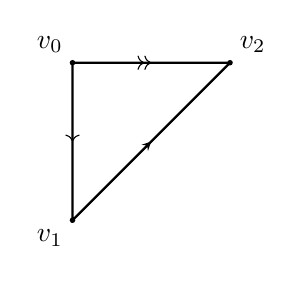
\begin{tikzpicture}[scale=2]
	\fill (0,0) circle[radius=.5pt] node[below left]{$v_1$};
	\fill (0,1) circle[radius=.5pt] node[above left]{$v_0$};
	\fill (1,1) circle[radius=.5pt] node[above right]{$v_2$};
	\draw[
    	decoration={markings, mark=at position 0.5 with {\arrow{>>}}},
		postaction={decorate},
		] (0,1) -- (1,1);
	\draw[
    	decoration={markings, mark=at position 0.5 with {\arrow{>}}},
		postaction={decorate}
		] (0,1) -- (0,0);
	\draw[
    	decoration={markings, mark=at position 0.5 with {\arrow{stealth}}},
		postaction={decorate}
		] (0,0) -- (1,1);
	\draw[thick] (0,0)--(0,1)--(1,1)--cycle;
\end{tikzpicture}

%% Torus_L (Homology-3.png)
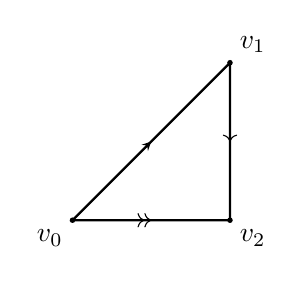
\begin{tikzpicture}[scale=2]
	\fill (0,0) circle[radius=.5pt] node[below left]{$v_0$};
	\fill (1,0) circle[radius=.5pt] node[below right]{$v_2$};
	\fill (1,1) circle[radius=.5pt] node[above right]{$v_1$};
	\draw[
    	decoration={markings, mark=at position 0.5 with {\arrow{>}}},
		postaction={decorate},
		] (1,1) -- (1,0);
	\draw[
    	decoration={markings, mark=at position 0.5 with {\arrow{>>}}},
		postaction={decorate}
		] (0,0) -- (1,0);
	\draw[
    	decoration={markings, mark=at position 0.5 with {\arrow{stealth}}},
		postaction={decorate}
		] (0,0) -- (1,1);
	\draw[thick] (0,0)--(1,0)--(1,1)--cycle;
\end{tikzpicture}